\documentclass{article}
\usepackage[utf8]{inputenc}
\usepackage{graphicx}
\usepackage{hyperref}
\hypersetup{
    colorlinks,
    citecolor=black,
    filecolor=black,
    linkcolor=black,
    urlcolor=black
}

\title{IMP - Hra na displej}
\author{Krištof Šiška (xsiska16)}
\date{December 2022}

\begin{document}

\maketitle

\section{Úvod}
Cieľom tejto práce bolo vytvoriť jednoduchú hru na displej I2C (128x64) za použitita platformy ESP32 a joysticku. Program bol vyvíjaný vo VScode za využitia doplňku platformio.

\subsection{Zapojenie}
    \begin{figure}[h!]
        \centering
        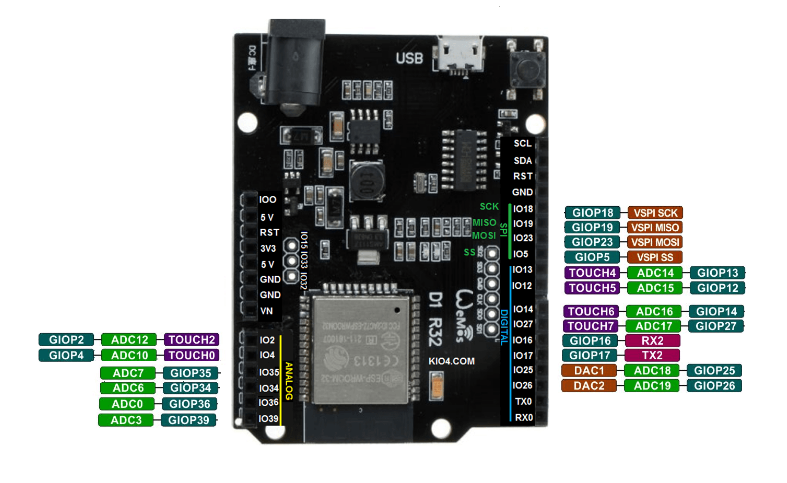
\includegraphics[scale=0.8]{ESP32.png}
        \caption{Schéma platformy ESP32}
    \end{figure} 
Displej I2C : 

    \begin{itemize}
        \item VCC $ \rightarrow $ +5V 
        \item GND $ \rightarrow $ GND
        \item SCL $ \rightarrow $ GIOP17
        \item SDA $ \rightarrow $ GIOP16
 \end{itemize}   
Joystick :

    \begin{itemize}
        \item GND $ \rightarrow $ GND
        \item +5V $ \rightarrow $ +3V3
        \item VRx $ \rightarrow $ ADC6
        \item VRy $ \rightarrow $ ADC7
        \item SW $ \rightarrow \emptyset $ 
    \end{itemize}
Zapojenie SW pinu joysticku nebolo nutné riešiť, keďže vymyslená hra
pracuje len s rýchlosťou a smerom pohybu a na stlačenie joystick tlačítka
nereaguje.

\section{Popis riešenia}
Implementácia celého riešenie sa nachádza v súbore \verb|main.c|. Na začiatku sa inicalizuje displej, nastavenie analógových vstupov a premenné popisujúce výskyt objektu na disppleji. Samotné chovanie programu sa nachádaza vo \verb|while| smyčke, ktorá je nekonečná. Každým cyklom sa prečíta aktuálna hodnota na analógových vstupoch, popisujúce smer a rýchlosť v smere X a Y osy. Pre jednoduchšiu prácu sú potom tieto hodnoty normalizované (pokiaľ je hodnota vačšia ako 3600, nastaví sa práve a túto hodnotu). Pri provtnej kalibrácií bolo zistené, že hodnota v pokoji joysticku (základná poloha) na vstupe pre X osu je približne 1817. Pre Y osu je to približne 1870. Pre malé výkyvy v čítaniach považujeme joystick v základnom stave pokiaľ hodnota na vstupe je v rozmedzí 1700 až 1900. Po zisťení smeru pohybu sa objekt na obrazovke posunie na daný smer pomocou funkcie \verb|ssd1306_wrap_arround|.
Rýchlosť je simulovaná pomocou čakania na vykonanie posunu. Pokiaľ je rýchlosť vysoká (joystick je v maximálnej alebo minimálnej polohe) čakanie na vykonanie pohybu sa blíži k nule. Naopak čim bližšie je joystick k stave pokoja, tým je čakanie dlhšie. Po vykonaní pohybu sa pomocou funkcie \verb|check_collisions| zistí, či objekt narazil do správneho rohu, pokiaľ sa tak stalo, hra sa premiestni do pôvodného stavu a vyberie sa nový cieľ pre ďaľšie kolo. 

\section{Záver}
Cieľom projektu bolo vytvoriť hru a ukázať správnu prácu s perifériami. Práca s joystickom je ukázaná na rýchlosti pohybu objektu. Riešenie v súčasnom stave obsahuje pár nedostatkov. Najznámejší z nich je ten, že hra dokáže správne kontrolovať kolíziu so správnou stranou jedine v prípade, že nedošlo v priebehu kola ku kolízií a následnému pretečeniu s inou stranou. Autor túto skutočnosť nepovažuje za príliš problematickú, keďže cieľom bolo ukázať správnu prácu s perifériami a nie vytvoriť dokonale funkčnú hru. Programové riešenie je čitateľné a zadanie bolo rozdelené do viacerých podproblémov.
V tomto dokumente nie sú vysvetlené pravidlá ani princípy hry,  keďže autor verí, že hra je po spustení na prvý pohľad zrozumiteľná a hráč zistí čo je cieľom hry sám. Ukážka cieľa je najlepšie ukázana na \href{https://drive.google.com/file/d/1UcCmRvFZmSy3YNQ0_3ex0Vm7ZOvGVgdJ/view?usp=sharing}{videu} .

\section{Autoevaluácia}
D - 2/4 \\
E - 1/1 \\
F - 5/5 \\ 
Q - 3/3 \\
P - 1/1 \\
Celkové hodnotenie : 12/14

\end{document}
